\documentclass[aspectratio=169]{beamer}

\usetheme{metropolis}
\usepackage{appendixnumberbeamer}

\usepackage{amsmath}
\usepackage{amssymb}
\usepackage{mathtools}
\usepackage{booktabs}
\usepackage{colortbl}
\usepackage{tikz}
\usepackage{pgfplots}
\pgfplotsset{compat=1.18}
\usepackage{graphicx}
\usepackage{subcaption}
\usepackage{algorithm}
\usepackage{algorithmic}

\graphicspath{{../Figures/}}

\definecolor{mkgreen}{RGB}{0,128,80}
\definecolor{nmblue}{RGB}{50,100,180}
\definecolor{alertorange}{RGB}{220,100,30}

\setbeamercolor{block title}{bg=mkgreen!20, fg=black}
\setbeamercolor{block body}{bg=mkgreen!5}

\title{Markovian Transformers for\\Informative Language Modeling}
\author{Scott W.\ Viteri \and Max Lamparth \and Peter Chatain \and Clark Barrett}
\institute{Stanford University}
\date{ICLR 2026}

\begin{document}

\begin{frame}[plain]
\maketitle
\end{frame}

\begin{frame}{Motivation: Why Ask the Model?}

\begin{columns}[T]
\column{0.55\textwidth}
\small
\textbf{The appealing dream}: interpretability by just asking the LM to explain its thinking.

\begin{itemize}
    \itemsep 0.15em
    \item We already speak natural language
    \item The model already speaks natural language
    \item The model has access to its own internal representations
\end{itemize}

But ordinary CoTs are often \alert{not faithful}:
\begin{itemize}
    \itemsep 0.15em
    \item Spurious biases can remain hidden
    \item Altering the CoT may not change the answer
    \item The model can \textbf{bypass} the CoT entirely
\end{itemize}

\column{0.42\textwidth}
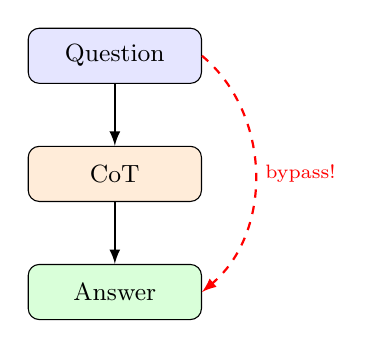
\begin{tikzpicture}[
    box/.style={rectangle, draw, rounded corners, minimum width=2.2cm,
                minimum height=0.7cm, font=\small},
    arrow/.style={->, thick, >=latex}
]
\node[box, fill=blue!10] (Q) at (0,3) {Question};
\node[box, fill=orange!15] (C) at (0,1.5) {CoT};
\node[box, fill=green!15] (A) at (0,0) {Answer};
\draw[arrow] (Q) -- (C);
\draw[arrow] (C) -- (A);
\draw[arrow, red, dashed, thick] (Q.east) to[bend left=50]
    node[right, font=\scriptsize, text=red]{bypass!} (A.east);
\end{tikzpicture}

\vspace{0.15cm}
{\small\color{red} Standard models can still see the question when generating the answer.}
\end{columns}
\end{frame}

\begin{frame}{Pragmatic Goal: Informative CoT}

\small
\textbf{Target}: the CoT alone should suffice for the answer.

\smallskip
\emph{Notecard intuition}: before you lose the question, write down the part of your understanding you will need later.

\begin{center}
\resizebox{0.68\textwidth}{!}{%
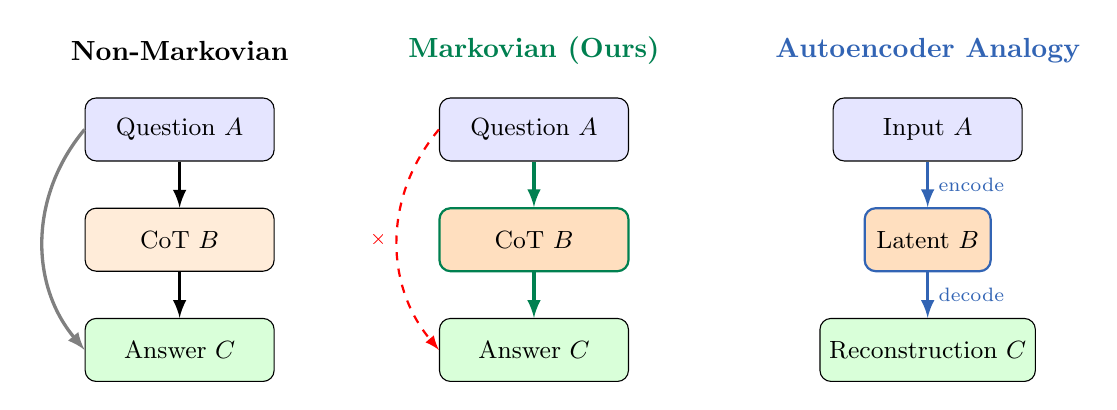
\begin{tikzpicture}[
    box/.style={rectangle, draw, rounded corners, minimum width=2.4cm,
                minimum height=0.8cm, font=\small},
    arrow/.style={->, very thick, >=latex}
]
\node[font=\bfseries] at (-4.5,3.2) {Non-Markovian};
\node[box, fill=blue!10] (Q1) at (-4.5,2.2) {Question $A$};
\node[box, fill=orange!15] (C1) at (-4.5,0.8) {CoT $B$};
\node[box, fill=green!15] (A1) at (-4.5,-0.6) {Answer $C$};
\draw[arrow] (Q1) -- (C1);
\draw[arrow] (C1) -- (A1);
\draw[arrow, gray] (Q1.west) to[bend right=40] (A1.west);

\node[font=\bfseries, text=mkgreen] at (0,3.2) {Markovian (Ours)};
\node[box, fill=blue!10] (Q2) at (0,2.2) {Question $A$};
\node[box, fill=orange!25, thick, draw=mkgreen] (C2) at (0,0.8) {CoT $B$};
\node[box, fill=green!15] (A2) at (0,-0.6) {Answer $C$};
\draw[arrow, mkgreen] (Q2) -- (C2);
\draw[arrow, mkgreen] (C2) -- (A2);
\draw[arrow, red, dashed, thick] (Q2.west) to[bend right=40]
    node[left, font=\scriptsize, text=red]{\texttimes} (A2.west);

\node[font=\bfseries, text=nmblue] at (5,3.2) {Autoencoder Analogy};
\node[box, fill=blue!10] (E) at (5,2.2) {Input $A$};
\node[box, fill=orange!25, thick, draw=nmblue,
      minimum width=1.6cm] (L) at (5,0.8) {Latent $B$};
\node[box, fill=green!15] (D) at (5,-0.6) {Reconstruction $C$};
\draw[arrow, nmblue] (E) -- node[right, font=\scriptsize]{encode} (L);
\draw[arrow, nmblue] (L) -- node[right, font=\scriptsize]{decode} (D);
\end{tikzpicture}
}
\end{center}

\vspace{-0.15cm}
\textbf{Bandwidth bottleneck}: all information from $A$ to $C$ must flow through $B$.

\smallskip
\footnotesize Autoencoder intuition: compress what matters into a note the model can still use later.
\end{frame}

\begin{frame}{Training: GRPO-Style Policy Gradient}

\textbf{Key innovation}: the reward $R_\theta$ depends on $\theta$, so we get two gradient terms:
\[
\nabla_\theta\, \mathbb{E}[R_\theta(\tau)]
:= \mathbb{E}\!\Big[\underbrace{R_\theta \cdot \nabla_\theta \ln P_\theta(\tau)}_{\text{policy gradient}}
  + \underbrace{\nabla_\theta R_\theta(\tau)}_{\text{actor-reward gradient}}\Big]
\]
\vspace{-0.35cm}

\textbf{Loss function}:
\[
\mathcal{L} = \underbrace{\mathcal{L}_{\text{PG}}}_{\text{REINFORCE}} + \underbrace{\mathcal{L}_{\text{AR}}}_{\text{direct reward}} + \underbrace{\mathcal{L}_{\text{KL}}}_{\text{regularization}}
\]
\vspace{-0.25cm}

\begin{itemize}
    \itemsep 0.2em
    \item \textbf{Parallel sampling}: multiple CoTs per question (GRPO-style)
    \item \textbf{Within-batch standardization}: advantages have zero mean, unit variance
    \item \textbf{KL penalty} ($\beta = 0.1$): discourages steganographic encodings
    \item \textbf{LoRA} (rank 8): stable fine-tuning with frozen base weights
\end{itemize}
\end{frame}

\begin{frame}{Performance and Load-Bearing CoTs}

\begin{columns}[T]
\column{0.49\textwidth}
\textbf{Performance stays competitive}

\begin{table}
\centering
\tiny
\setlength{\tabcolsep}{3pt}
\begin{tabular}{lccc}
\toprule
Task & Base & NM & Mkv \\
\midrule
GSM8K & 19.6 & 63.3 & 57.1 \\
ARC & 36.1 & 78.6 & 79.9 \\
Arith. & 1.0 & 97.0 & 98.0 \\
MMLU & 21.4 & 68.7 & 55.5 \\
SVAMP & 18.0 & 43.3 & 42.3 \\
\midrule
Avg. & 19.2 & 70.2 & 66.6 \\
\bottomrule
\end{tabular}
\end{table}

\begin{itemize}
    \itemsep 0.15em
    \item Large gains over the base model
    \item Usually close to Non-Markovian
\end{itemize}

\column{0.49\textwidth}
\textbf{CoT becomes load-bearing}

\begin{table}
\centering
\scriptsize
\begin{tabular}{lc}
\toprule
Perturbation & $\Delta \ln P$ \\
\midrule
Delete & +0.926 \\
Char Repl. & +0.902 \\
Trunc. Back & +0.699 \\
Trunc. Front & +0.456 \\
\bottomrule
\end{tabular}
\end{table}

\vspace{0.05cm}
\scriptsize Exact Figure 2 wiki sensitivity values. Positive means the Markovian model is more fragile to CoT corruption, hence more reliant on the CoT.
\end{columns}

\vspace{0.1cm}
\begin{center}
\colorbox{mkgreen!10}{\parbox{0.9\textwidth}{\centering
Most of the performance remains, and the CoT becomes causally essential.
}}
\end{center}
\end{frame}

\begin{frame}{Cross-Model Transfer: CoTs Generalize}

\textbf{Question}: are trained CoTs only useful to the model that produced them?

\bigskip
\textbf{Finding}: no.

\begin{itemize}
    \item CoTs trained under the Markovian bottleneck transfer across different critics
    \item Gains are visible even for very different architectures and scales
    \item Transfer to \textbf{GPT-2} is especially important: a small model should not be able to decode sophisticated steganography
\end{itemize}

\bigskip
\begin{center}
\colorbox{mkgreen!10}{\parbox{0.82\textwidth}{\centering
Cross-model usefulness supports the claim that the CoTs contain ordinary natural-language reasoning, not model-specific codes.
}}
\end{center}
\end{frame}

\begin{frame}{Summary}

\begin{enumerate}
    \item \textbf{Markovian framework}: answer prediction must go through the CoT
    \item \textbf{Training}: GRPO-style sampling plus actor-reward gradients and KL regularization
    \item \textbf{Performance}: strong gains over the base model, competitive with Non-Markovian
    \item \textbf{Interpretability evidence}: perturbation fragility and cross-model transfer both support load-bearing CoTs
\end{enumerate}

\vspace{0.3cm}
\begin{center}
\Large Thank you!

\normalsize
Code: \texttt{github.com/scottviteri/MarkovianTraining}
\end{center}
\end{frame}

\end{document}
